% !TEX root = ../notes.tex

\begin{titlepage} %Titre
\begin{center}
\newcommand{\HRule}{\rule{\linewidth}{0.5mm}} % Defines a new command for the horizontal lines, change thickness here
\center % Center everything on the page
 
 
 %----------------------------------------------------------------------------------------
% TITLE SECTION
%----------------------------------------------------------------------------------------




\begin{figure} [h] %----------- SubGraph ---------------------
\centerline{
\subfigure{
\includegraphics[height = 2 cm]{./pic/EPFL.png}  }
\subfigure{
\includegraphics[height = 2 cm]{./pic/ADA-logo.png}} 
} 
\end{figure}


\vspace{0.5cm}
%\textsc{\LARGE EPFL}\\[1.5cm] % Name of your university/college
\textsc{\Large School of Computer and Communication Sciences}\\[0.5cm] % Major heading such as course name
\textsc{\Large }\\% Minor heading such as course title
%\textsc{ \Large Master Semester Project}\\ % Minor heading such as course title


\HRule \\[0.4cm]
{ \huge \bfseries Applied Data Analysis \\Summary}\\[0.4cm] % Title of your document
\HRule \\[1.5cm]

% ---- Lovelace -----
\begin{center}
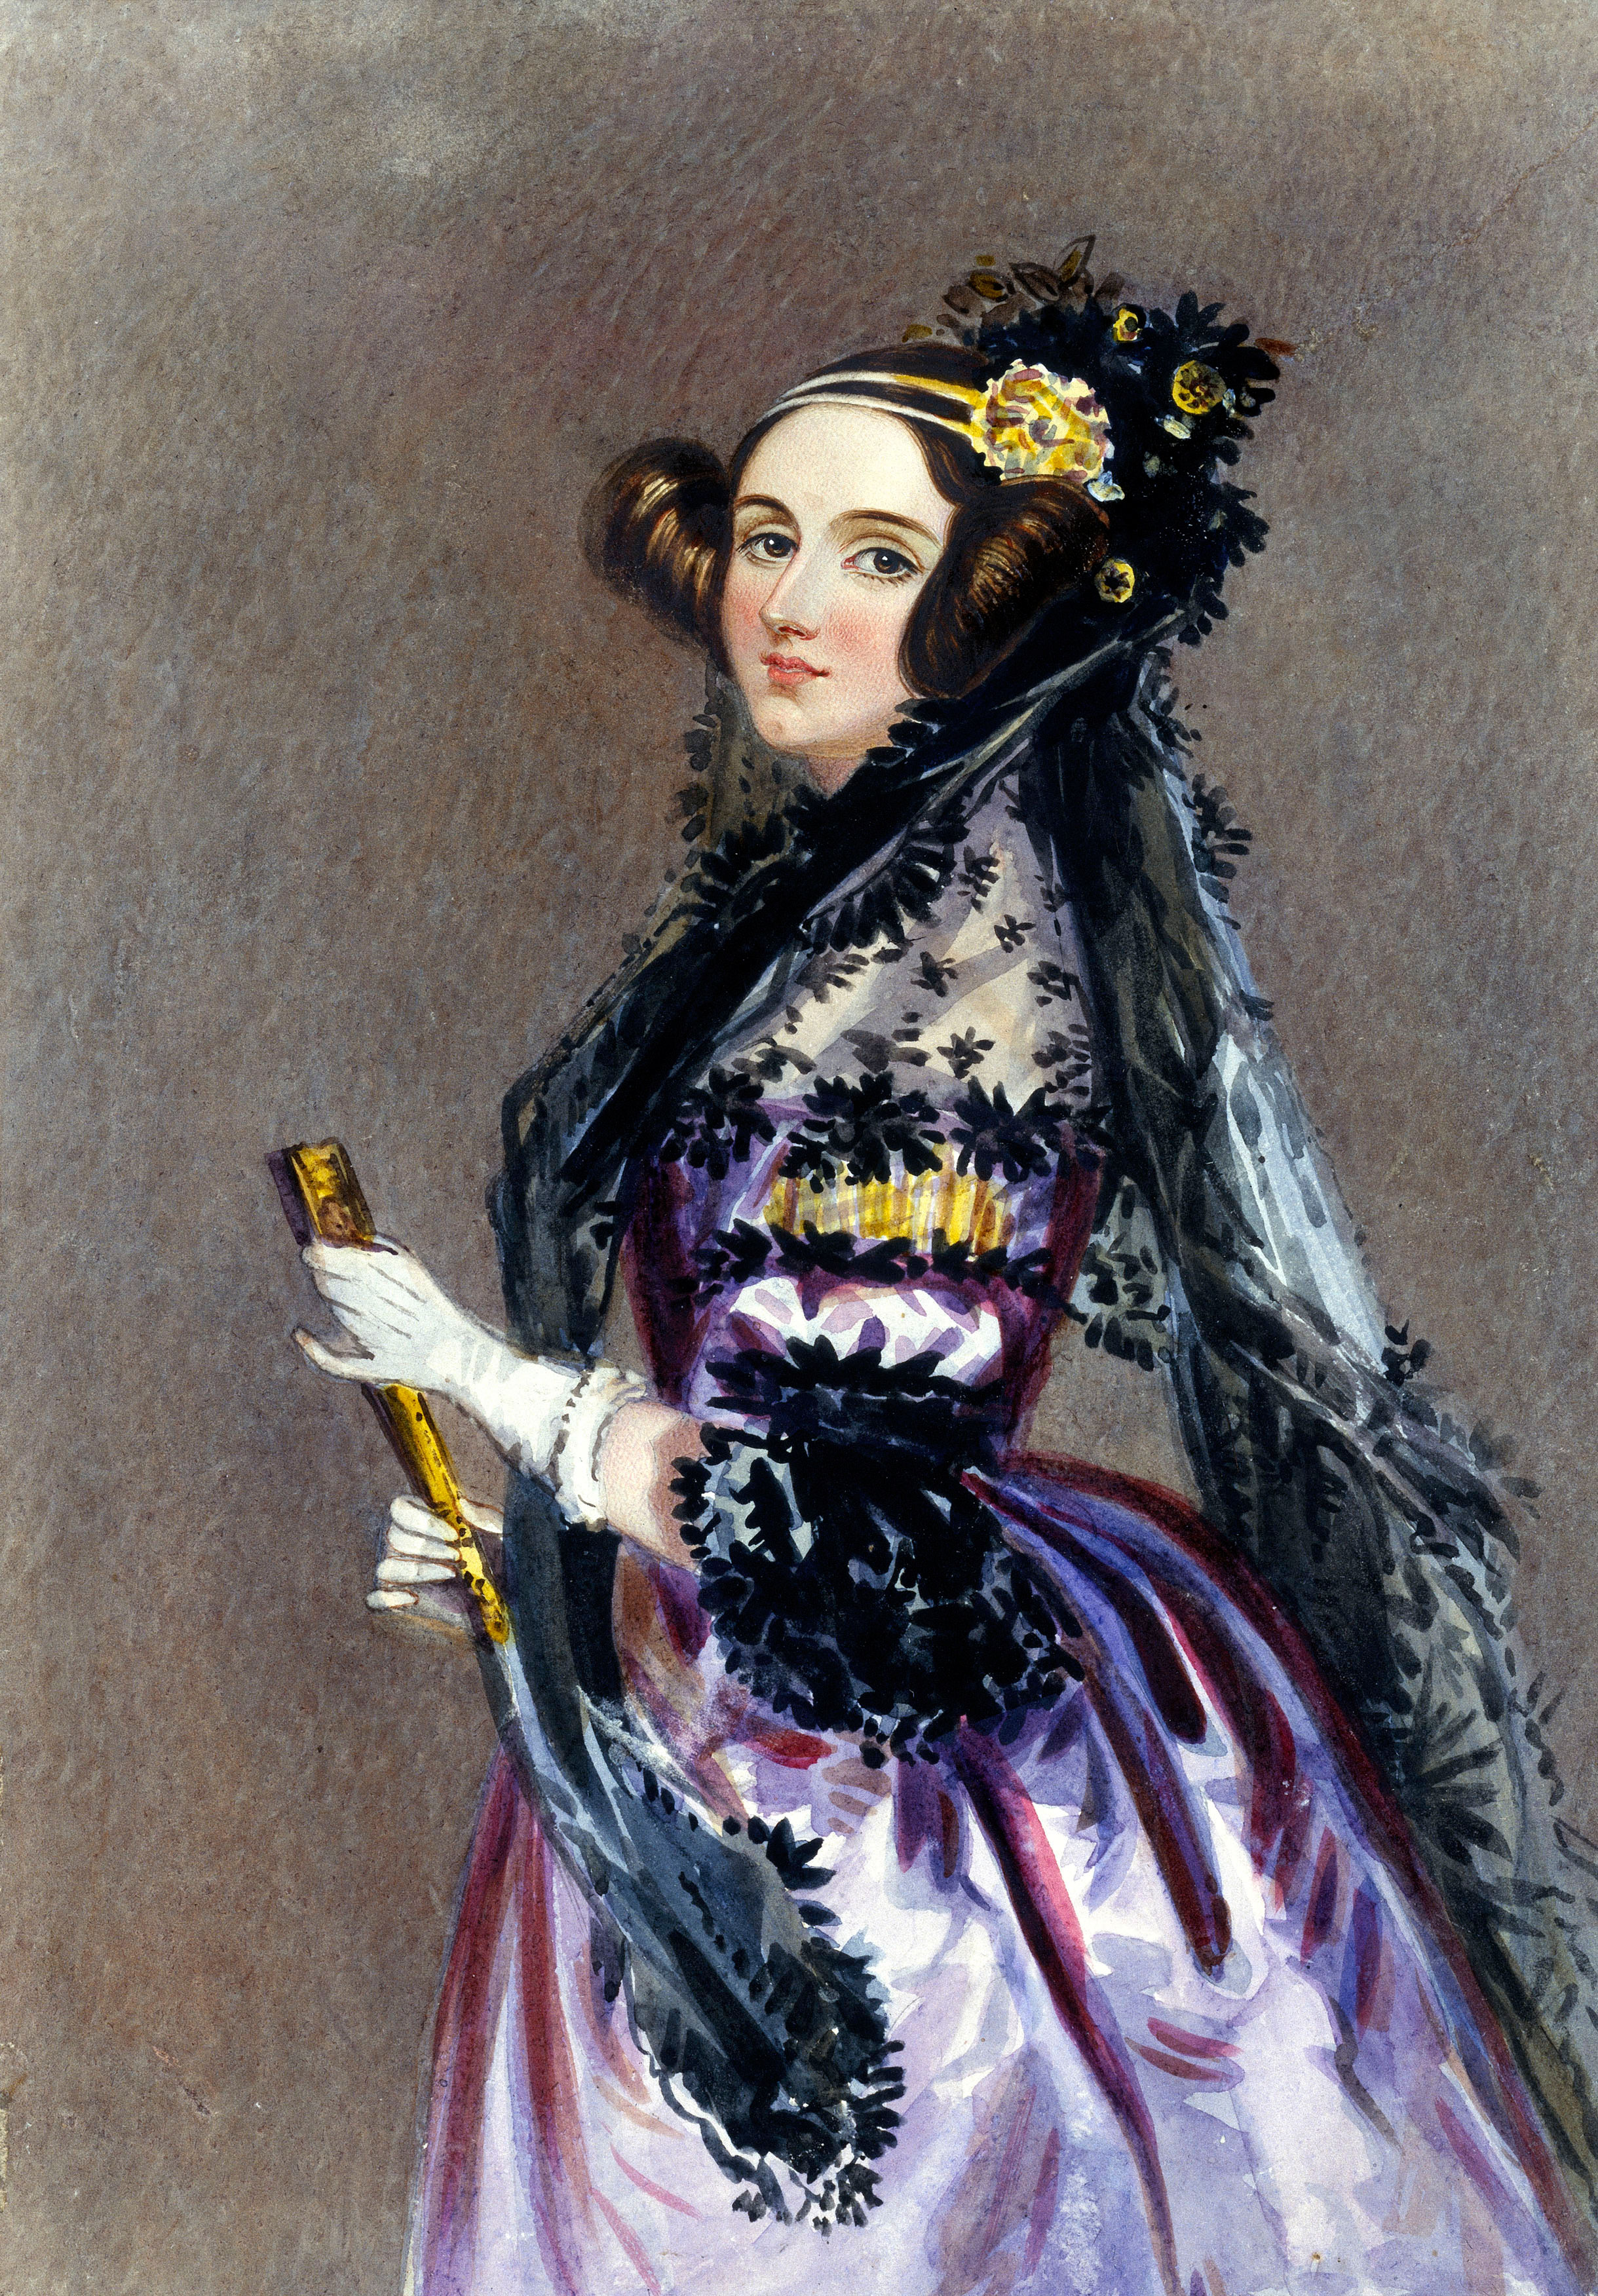
\includegraphics[width = 5 cm]{pic/lovelace} % Include a department/university logo - this will require the graphicx package
\end{center}



\begin{bottompar}
% ---- Professor -----
\begin{flushleft} \large
Dr. \textsc{Catasta} Michele\\
Distributed Information Systems Laboratory (LSIR) \\
\mail{michele.catasta@epfl.ch} \\ 
\end{flushleft}

% ---- date
{\large June 10, 2016}\\[1cm] % Date, change the \today to a set date if you want to be precise

\end{bottompar}
 
\vfill % Fill the rest of the page with whitespace

\end{center}
\end{titlepage}

\clearpage